
% ================= DEIMOS USE CASE =================

Telemetry and flight instrumentation are essential
for launch vehicles, spacecraft, and experimental
aerospace platforms. NASA's Artemis I mission
utilized extensive flight instrumentation to
record and transmit engineering measurements,
enabling the validation of launch vehicle models
and evaluation of flight performance
\cite{NASA_Artemis_Instrumentation}.

The \deimos{} subsystem applies these principles
through onboard data acquisition, flight orientation
measurements, and wireless telemetry. Its development
supports applications in spacecraft monitoring,
experimental flight testing, and autonomous
aerospace instrumentation.

\begin{figure}[H]
    \centering
    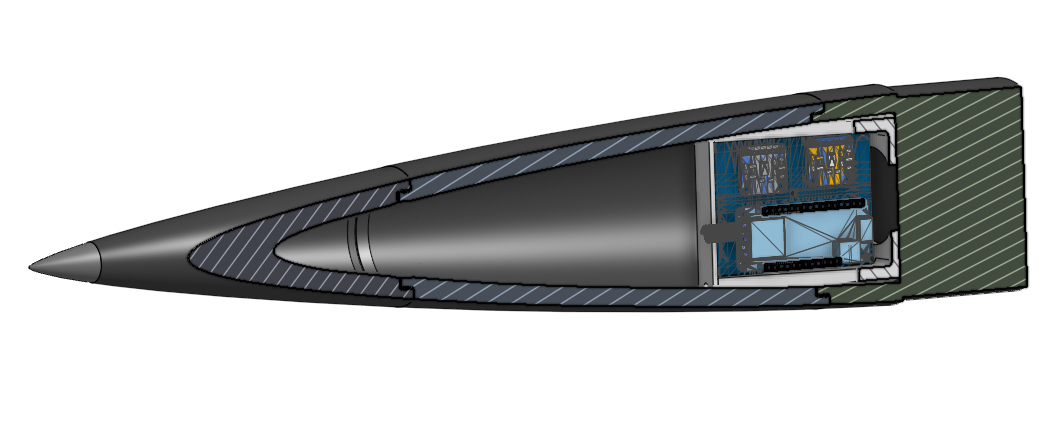
\includegraphics[width=1\linewidth]{Documentation/ARES/Use_Cases/Pics/DEIMOS_CAD.png}
    \caption{\deimos{} CAD Model housed within Nose Cone.}
    \label{fig:placeholder}
\end{figure}